\secnumbersection{MARCO CONCEPTUAL}

Para abordar nuestro problema, primero debemos definir algunos conceptos que han
sido mencionados en las secciones anteriores de forma más formal, tales como, la
web semántica, \textit{SPARQL}, \textit{RDF} y el contexto en el que estos se
utilizan. Para esto, nos apoyaremos en las siguientes definiciones.

\subsection{Web Semántica}

La red informática mundial, \textit{World Wide Web} o simplemente \textit{Web}
es el sistema de información público más importante desarrollado en los últimos
30 años, el cual permite la transmisión de documentos electrónicos identificados
por URIs \textit{(Uniform Resource Identifiers)}, los cuales pueden estar
enlazados a otros documentos a través de hipertexto y que se encuentran
disponibles utilizando servicios de la internet.

La \textit{World Wide Web} fue diseñada como un espacio para la información con
el objetivo de no solo ser útil para las comunicaciones entre humanos, sino que
también un lugar donde las máquinas podrían ayudar y participar. Sin embargo,
uno de los principales problemas de la \textit{Web} es que la mayor parte de su
contenido ha sido diseñado para ser consumido por humanos, lo que implica que
para las máquinas y el software no es fácil acceder e interpretar el contenido
disponible, incluso si este proviene de una base de datos estructurada a través
de columnas claras y tipificadas. La web semántica busca desarrollar
herramientas, lenguajes, protocolos y estándares que permitan, tanto a maquinas
como humanos, procesar toda la información disponible en la \textit{Web}. En
base a esto, podemos definir a la web semántica como la idea de generar una red
de datos en la \textit{Web}, hasta cierto punto, una base de datos global.
\cite{berners1998semantic}

\subsection{Arquitectura de la web semántica}

La web semántica está construida en base a múltiples bloques, los cuales
representan estándares y lenguajes utilizados para lograr determinadas
funcionalidades descritas en su arquitectura \cite{harth2011semantic}, una
representación gráfica de esta arquitectura en bloques se puede observar en la
figura \ref{fig:semantic-web-arq}, la cual, podemos describir en las siguientes
capas.

\begin{figure}
    \label{fig:semantic-web-arq}
    \centering
    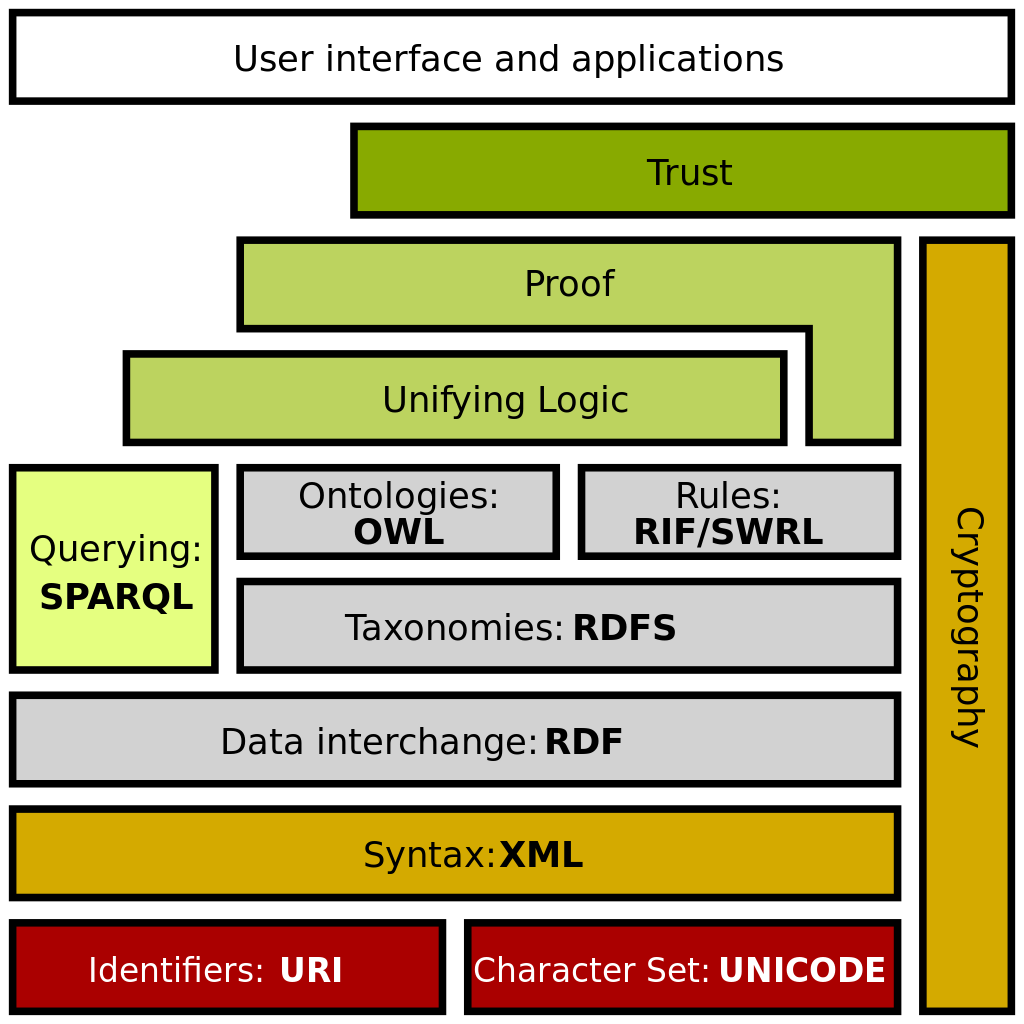
\includegraphics[width=0.6\linewidth]{semantic_web_stack}
    \caption{Arquitectura de la web semántica.} Fuente: FIXME
\end{figure}

\subsubsection{Referencias, transporte y principios de los datos enlazados}

El acceso a los datos es fundamental para la arquitectura de la web semántica.
Podemos tomar como referencia, el modelo utilizado por los servidores
\textit{Web}, en el cual, los documentos disponibles se encuentran enlazados a
otros de forma descentralizada, esto es, que el documento referenciado no
necesariamente se encuentra en el mismo servidor que está haciendo referencia a
él. Estos enlaces, son utilizados por los usuarios para navegar entre los
millones de servidores disponibles en la \textit{Web}.

Las URI/IRI y el protocolo HTTP son parte fundamental del
núcleo que define tanto a la \textit{World Wide Web} como a la web semántica. En
un ejemplo concreto, la URI
\url{https://en.wikipedia.org/wiki/Back_to_the_Future} en la \textit{Web},
representa el documento en el servidor \url{https://www.wikipedia.org} que contiene
información sobre la serie de películas y obras de título ``Volver al Futuro'',
en cambio, en el contexto de la web semántica, la URI
\url{https://www.wikidata.org/wiki/Q1} representa al ``universo'' como una
entidad, la cual es parte del \url{https://www.wikidata.org/wiki/Q3327819}
``multiverso'' y es estudiado por la \url{https://www.wikidata.org/wiki/Q338}
``cosmología''.

Los datos del ejemplo anterior son publicados por ``The Wikipedia
Fundation" a través del servicio Wikidata
\cite{vrandevcic2014wikidata}, pero las relaciones descritas podrían enlazar a
otros editores de contenido, como por ejemplo DBpedia
\cite{valsecchi2015dbpedia}, el cual es un esfuerzo comunitario para extraer
información estructurada desde distintas fuentes y enlazarlas a través del
formato \textit{RDF}. Para lograr esto, los editores de contenido para la web semántica
aplican los siguientes principios a sus datos, los cuales son conocidos como los
``principios para datos enlazados'' o \textit{LinkedData principles}
\cite{bizer2011linked}.

\begin{enumerate}
    \item Usar URIs como nombres para entidades.
    \item Usar UIRs HTTP para que los usuarios puedan buscar y acceder
    a estas entidades.
    \item Cuando un usuario consulta una URI, debes entregar
    información relevante, utilizando estándares como \textit{RDF} y \textit{SPARQL}.
    \item Debes incluir enlaces a otras URIs, para que los usuarios
    descubran más entidades.
\end{enumerate}

\subsubsection{Intercambio de datos}

\begin{figure}
    \label{fig:rdf-graph1}
    \centering
    \includesvg[width=\linewidth]{rdf-graph.svg}
    \caption{Un grafo \textit{RDF} básico.} Los nodos \textit{Subject} y \textit{Object}
    están conectados a través de la relación \textit{Predicate}. Fuente: FIXME.
\end{figure}

Los datos de la web semántica son generados por distintas entidades al rededor
del mundo, las cuales no están necesariamente coordinados entre ellos, por lo
que la arquitectura debe soportar la creación distribuida de datos junto con la
integración de múltiples fuentes y la interoperabilidad entre los datos creados
\cite{bizer2011linked}. Este tipo de requerimientos los cumplen las estructuras
de datos basados en grafos como \textit{RDF}. \textit{RDF} es un formato basado en la
descripción de grafos dirigidos, los cuales representan la información de la
forma de tríos sujeto - predicado - objeto, en la cual, el
sujeto y el predicado corresponden a nodos del grafo y el
predicado es un arco que los relaciona como se puede observar en la
figura \ref{fig:rdf-graph1}. En estos tríos, cualquiera de estos objetos puede
tomar el valor de una URI, un valor literal (cadenas de texto, números
o fechas) o simplemente un nodo vacío (identificadores que no pueden ser
referenciados por otra entidad).

\textit{RDF} corresponde a la especificación de un lenguaje abstracto para describir
relaciones entre entidades, el cual, puede ser serializado en múltiples formatos
de texto como \textit{Extensible Markup Language (XML)} \cite{beckett2004rdf}
(listing \ref{lst:rdf-xml1}) o en un formato más compacto como \textit{Turtle}
\cite{beckett2014rdf} (listing \ref{lst:rdf-turtle}).

% \begin{lstlisting}[language=xml, captionpos=b, caption=Descripción de un documento en \textit{RDF/XML}, label=lst:rdf-xml1, basicstyle=\ttfamily, frame=single]
% <rdf:Description rdf:about="http://www.w3.org/TR/rdf-syntax-grammar"
%     dc:title="RDF 1.1 XML Syntax"> <ex:editor> <rdf:Description
%     ex:fullName="Dave Beckett"> <ex:homePage
%     rdf:resource="http://purl.org/net/dajobe/"/> </rdf:Description> </ex:editor>
% </rdf:Description>
% \end{lstlisting}


\begin{figure}
    \label{fig:rdf-turtle-ex}
    \centering
    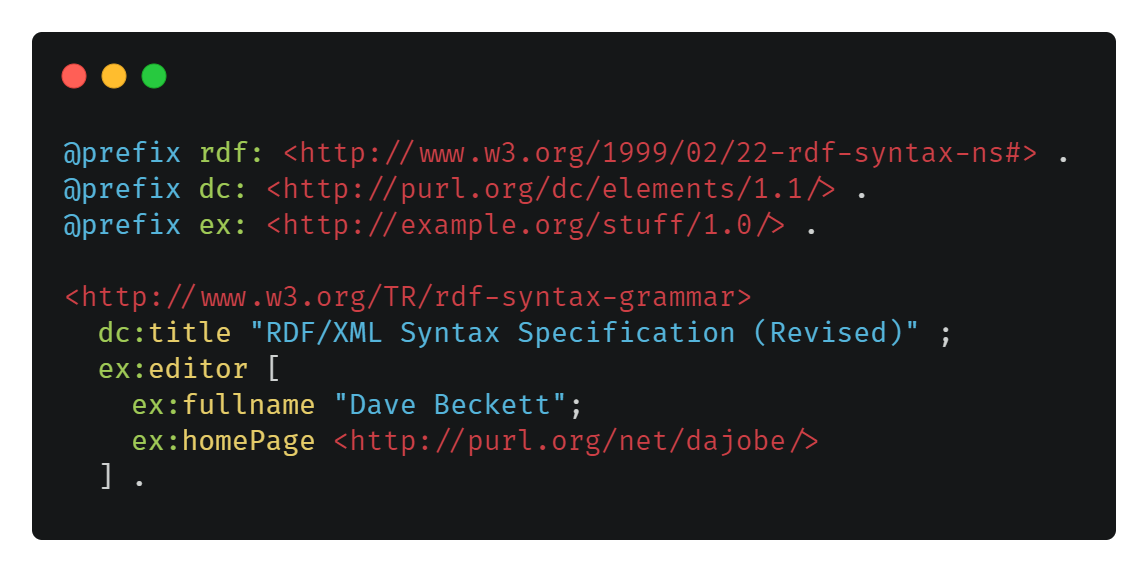
\includegraphics[width=\linewidth]{rdf-turtle-ex.png}
    \caption{Descripción de un documento \textit{RDF/Turtle}.} Fuente: Turtle
    (Syntax). Wikipedia.
\end{figure}

\subsubsection{Consultas y actualizaciones}

\subsubsection{Ontologías y razonamiento}

\subsubsection{Reglas}

\subsubsection{Seguridad y encriptación}

\subsubsection{Unificación e integración}

\subsubsection{Confianza}

\subsubsection{Aplicaciones}